\documentclass[]{article}
\usepackage[utf8]{inputenc}
\usepackage{amsmath}
\usepackage{amssymb}
\usepackage{graphicx}
\usepackage{geometry}
\usepackage{enumitem}
\usepackage{amsthm}
\usepackage{graphicx}
\usepackage{geometry}

\geometry{hmargin=2cm}

\title{Logique}

\author{Arnaud Durand et Pierre Gervais}

% Environnement type théorème
\newtheorem{mythm}{Théorème}
\newtheorem{myproposition}{Proposition}
\newtheorem{myproperty}{Propriété}
\newtheorem{mylemma}{Lemme}
\newtheorem{mycor}{Corollaire}

% Environnement type texte
\theoremstyle{remark}
\newtheorem{mynot}{Notation}
\newtheorem{myrem}{Remarque}
\newtheorem{myexer}{Exercice}
\newtheorem{myproof}{Preuve}
\newtheorem{myexmpl}{Exemple}

% Environnement de définition
\theoremstyle{definition}
\newtheorem{mydef}{Définition}

\setlist[itemize]{label=-}

% Carré de fin de preuve
\newcommand{\cqfd}{
	\hfill$\square$
}

% "Checkmark" de fin d'étape de preuve
\newcommand{\checked}{
	\hfill$\checkmark$
}

% Définition de fonction
\newcommand{\func}[5]{
#1 ~ : ~ \left\{ \begin{array}{lcl}
	#2 & \longrightarrow & #3 \\
	#4 & \longmapsto & #5
\end{array}
\right.
}

\newcommand{\funcinline}[5]{
#1 ~ : ~ #2 \longrightarrow #3, ~ #4 \longmapsto #5
}

\newcommand{\funcshort}[3]{
#1 ~ : ~ #2 \longrightarrow #3
}

\newenvironment{proofpart}[1]{
	\leavevmode
	
	\noindent
	{\textit{\textbf{\boldmath #1}}}
	
}{
	\checkmark
}

\begin{document}

\maketitle

\tableofcontents

\part{Calcul propositionnel}

\section{Syntaxe}

Le \textit{calcul propositionnel} est un langage \textit{inductivement} et \textit{librement engendré} par un ensemble de règles.

C'est à dire qu'une formule ne peut pas être obtenu de deux façons différentes.

\begin{mydef}	
	Soit $\mathcal{P}$ un ensemble de constantes propositionnelles, on définit $\mathcal{F}_\mathcal{P}$ le calcul propositionnel sur $\mathcal{P}$ obtenu par les règles suivantes :
	\begin{itemize}
		\item si $p \in \mathcal{P}$, alors $p \in \mathcal{F}_\mathcal{P}$
		
		\item $\perp \in \mathcal{F}_\mathcal{P}$
		
		\item si $F \in \mathcal{F}_\mathcal{P}$, alors $\left(\neg F\right) \in \mathcal{F}_\mathcal{P}$
		
		\item si $F, G \in \mathcal{F}_\mathcal{P}$ alors $(F \lor G), (F \land G), (F \rightarrow G) \in \mathcal{F}_\mathcal{P}$
	\end{itemize}
\end{mydef}

\begin{mynot}
	S'il n'y a pas d'ambiguïté, on notera $\mathcal{F}_\mathcal{P} = \mathcal{F}$
\end{mynot}

\begin{mydef}
	Une définition alternative de $\mathcal{F}$ est $\displaystyle \mathcal{F} = \bigcup_{n \geqslant 0} \mathcal{F}_n$
	où
	\begin{itemize}
		\item $\mathcal{F}_0 = \mathcal{P}$
		\item $\mathcal{F}_{n+1} = \mathcal{F}_n \cup \{(\neg F) ~ | ~ F \in \mathcal{F}_n)\} \cup \{(F \star G) ~ | ~ F, G \in \mathcal{F}_n, ~ \star \in \{\land, \lor, \rightarrow\}\}$, avec $n \geqslant 0$
	\end{itemize}
	
	On définit la \textit{hauteur} d'une formule $F$ par le plus petit $n$ tel que $F \in \mathcal{F}_n$.
\end{mydef}

\begin{myrem}
	Ce langage est fortement parenthésé et toute formule peut être représentée par un arbre de décomposition.
\end{myrem}

\begin{figure}[h!]
	\centering
	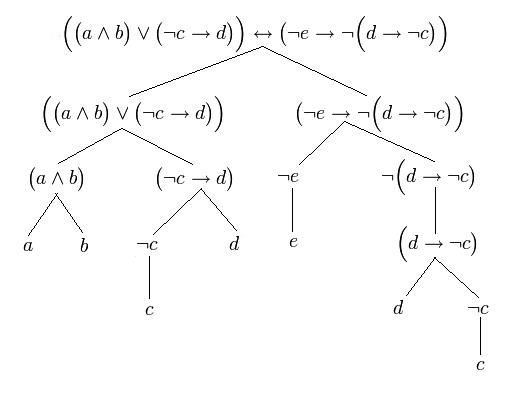
\includegraphics{Arbre_decomposition}
	\caption{Arbre de décomposition}
\end{figure}

\begin{myproperty}{Propriété de lecture unique}

	Pour tout $F \in \mathcal{F}$, un seul de ces cas est vrai :
	
	\begin{enumerate}
		\item $F \in \mathcal{P}$
		\item Il existe un \textit{unique} $G \in \mathcal{F}$ tel que $F = (\neg G)$

		\item Il existe d'\textit{uniques} $G,H \in \mathcal{F}$ et $\star \in \{\lor, \land, \rightarrow \}$ tels que $F = G \star H$
	\end{enumerate}

	C'est-à-dire que toute formule ne peut se décomposer que d'une seule façon.
\end{myproperty}

\subsection{Raisonnements}

On démontrera généralement les propriétés s'appliquant à $\mathcal{F}$ par induction :
pour démontrer une proposition $A$ s'appliquant à $\mathcal{F}$, on la démontre sur $\mathcal{P}$ et pour tout $(F \star G)$ et $(\neg F)$ où on suppose que $F, G \in \mathcal{F}$ vérifient $A$ et $\star \in \{\land, \lor, \rightarrow\}.$

\subsection{Définition alternative de $\mathcal{F}_\mathcal{P}$}

Soit $\Sigma = \mathcal{P} \cup \{(, ), \neg, \land, \lor, \rightarrow, \perp \}$, $\Sigma^*$ est l'ensemble des mots sur $\Sigma$.

\begin{myexmpl}
	\leavevmode
	\begin{itemize}
		\item $F = (\land \neg x_1)(( \in \Sigma^*$
		\item $F = (\neg x_1) \in \Sigma^*$
	\end{itemize}
\end{myexmpl}

\begin{mydef}
	$\mathcal{F}$ est le plus petit sous-ensemble de $\Sigma^*$ contenant $\mathcal{P} \cup \{\perp\}$ et \textbf{clos} par les opérations
	\begin{enumerate}
		\item $(F, G) \longmapsto (F \lor G)$
		\item $(F, G) \longmapsto (F \land G)$
		\item $(F, G) \longmapsto (F \rightarrow G)$
	\end{enumerate}
\end{mydef}

\begin{myrem}
	On peut montrer que les deux définitions correspondent.
	$\mathcal{F}$ satisfait la propriété de lecture unique (voir TD). 
\end{myrem}

\subsubsection{Sous-formule, hauteur, arbre de décomposition}

\begin{mydef}
	Soit $F \in \mathcal{F}$, on définit $\mathcal{S}(F)$ l'ensemble des \textit{sous-formules de $F$} telles que
	
	\begin{itemize}
		\item si $F \in \mathcal{P}$, $\mathcal{S}(F) = \{F\}$
		\item si $F = (\neg G)$ alors $\mathcal{S}(F) = \{F \} \cup \mathcal{S}(G)$
		\item si $F = (G \star H)$ où $\star \in \{\land, \lor, \rightarrow \}$, alors $\mathcal{S}(F) = \{F\} \cup \mathcal{S}(G) \cup \mathcal{S}(H)$
	\end{itemize}
\end{mydef}

TODO : vérifier dernier point

\begin{mydef}
	Soit $F \in \mathcal{F}$ on définit la \textit{hauteur} $h(F)$ de $F$ par
	\begin{itemize}
		\item $h(F) = 0$, si $F \in \mathcal{P}$
		\item si $=(\neg G)$, alors $h(F) = 1 + h(G)$
		\item si $F = (G \star H)$, alors $h(F) = 1 + \max\{h(G), h(H)\}$
	\end{itemize}
\end{mydef}

\begin{mydef}
	Soit $F \in \mathcal{F}$, l'\textit{arbre de décomposition de $F$} $arb(F)$ est un graphe étiqueté défini par
	
	\begin{enumerate}
		\item si $F \in \mathcal{P}$, $arb(F)$ est réduit à un sommet étiqueté par $F$.
		\item si $F = (\neg G)$, alors $arb(F) = \neg - arb(G)$
		\item si $F = (G \star H)$, alors $arb(F) = G - \star - H$
	\end{enumerate}
\end{mydef}

\begin{mynot}
	Soit $F$ une formule, $var(F)$ est l'ensemble des variables de $F$, $occ(F)$ est le multi-ensemble des variables de $F$ et $arb(F)$ est le graphe
	\begin{itemize}
		\item dont les sommets sont $V$
		\item et muni d'une fonction d'étiquetage $\lambda ~ : ~ V \longrightarrow \{\neg, \perp, \lor, \land, \rightarrow \} \cup var(F)$.
	\end{itemize}
\end{mynot}

\begin{myrem}
	Toutes les définitions sont univoques par la propriété de lecture unique.
\end{myrem}

\begin{myrem}
	On définit la hauteur d'une formule par la hauteur de son arbre de décomposition, c'est-à-dire la distance maximum entre les feuilles et la racine. 
\end{myrem}

\begin{mynot}
	\leavevmode
	\begin{itemize}
		\item $\top$ comme abréviation pour $(\perp \rightarrow \perp)$
		\item $(p \longleftrightarrow q)$ pour $(p \leftarrow q) \land (p \rightarrow q)$
		\item $\bigwedge\limits_{i=1}^n A_i = (((A_1 \land A_2) \land A_3)... \land A_n)$
	\end{itemize}
\end{mynot}

\section{Sémantique}

On s'intéresse à des propositions dont la valeur de vérité est soit vrai soit faux. On a besoin d'une \textbf{interprétation} (en terme de vrai ou faux) de ces constantes propositionnelles.

\begin{mydef}
	Une \textit{valuation} est une fonction $v ~ : ~ \mathcal{P} \longrightarrow \{0, 1\}$.
	Étant donné une valuation $v$, on définit l'\textit{interprétation} $\funcshort{\overline{v}}{\mathcal{F}}{\{0, 1\}}$ comme ceci
	\begin{itemize}
		\item si $F = p \in \mathcal{P}$ alors $\overline{v}=v(p)$
		\item si $F = (\neg G) \in \mathcal{P}$ alors $\overline{v}(F) = 1$ si et seulement si $\overline{v}(G) = 0$
		\item $\overline{v}(\perp)=0$
		\item $\overline{v}(F \land G) = 1$ si et seulement si $\overline{v} (F) = \overline{v} (G) = 1$
	\end{itemize}
\end{mydef}

On peut décrire l'interprétation d'une formule par sa \textit{table de vérité} :

$$
	\begin{array}{|c|c||c|c|c|}
		\hline
		F & G & \neg G & F \land G & F \rightarrow G \\
		\hline
		0 & 0 & 1 & 0 & 1 \\
		\hline
		0 & 1 & 1 & 0 & 1 \\
		\hline
	\end{array}
$$

On définit formellement la \textit{table de vérité} par une fonction $\funcshort{v}{\{0, 1\}^\mathcal{P}}{\{0, 1\}}$

\begin{mydef}
	\leavevmode
	\begin{itemize}
		\item $F \in \mathcal{F}$ est dit \textit{satisfaisable} s'il existe une valuation $v$ de $\mathcal{P}$ tel que $\overline{v}(F)=1$
		\item $F$ est dit \textit{valide} si pour toute valuation $v$ de $\mathcal{P}$, $\overline{v}(F) = 1$, on dit aussi que $F$ est une \textit{tautologie}.
		\item $F$ et $G$ sont dites \textit{équivalentes}, notées $F \equiv G$, si pour toute valuation $v$, $\overline{v}(F)=\overline{v}(G)$
		\item On note $v \models F \Longleftrightarrow \overline{v}(F)=1$, c'est à dire si et seulement si $v$ satisfait $F$.
	\end{itemize}
\end{mydef}

\begin{myexer}
	Vérifier que $F \equiv G$ si et seulement si $F \leftrightarrow G$ est valide.
\end{myexer}

\begin{myproposition}
	Pour tout $F \in \mathcal{F}$, $F$ est satisfaisable si et seulement si $(\neg F)$ n'est pas valide.
\end{myproposition}

\section{Exemples de formalisation}

\subsection{Contraites de compatibilité/exclusion}

\paragraph{Problème :}On possède $n$ produits chimiques à ranger dans $k \leqslant n$ conteneurs. Certains produits ne peuvent pas être stockés ensemble dans un conteneur.

La contrainte est donnée sous la forme d'un ensemble $\mathcal{L} \subseteq [n]$ tel que $I = \{i_1, ..., i_k\} \subseteq \mathcal{L}$ si et seulement si les produits $i_1, .., i_k$ ne peuvent pas être stockés ensemble.

\paragraph{Enjeu :}
Écrire une formule propositionnelle $F$ telle que $F$ est satisfaisable si le problème a une solution.

Les variables propositionnelles $\mathcal{P}=p(i, j), ~ i \leqslant n, ~ j \leqslant k$ sont interprétées par "le produit chimique $i$ est dans le camion $j$".

On exprime deux propositions :
\begin{itemize}
	\item Chaque produit se trouve dans un unique conteneur :
	$F = \underbrace{\left(\bigwedge\limits_{i \leqslant n} \left(\bigvee\limits_{j \leqslant k} p(i, j)\right) \right)}_{\substack{\text{Chaque produit } i \text{ est stocké} \\ \text{dans au moins un camion } j}} \land
	\underbrace{\left(\bigwedge\limits_{i \leqslant n} \left(\bigwedge\limits_{\substack{j, j' \leqslant k \\ j \neq j'}}(\neg\left(p(i, j) \land p(i, j')\right))\right)\right)}_{\substack{\text{Pour chaque produit } i \\ \text{ et chaque paire de camions } j \neq j' \\ \text{ il est faux que  } i \text{ est à la fois dans } j \text{ et } j'}}$
	
	\item On respecte les incompatibilités : $G = \underbrace{\bigwedge\limits_{I \subseteq \mathcal{L}} \left( \bigwedge\limits_{j \leqslant k}\neg \left( \bigwedge\limits_{i \in I}p(i, j)\right)\right)}_{\substack{\text{Pour chaque ensemble } I \text{ de produits } \\ \text{ne pouvant pas être stockés ensemble} \\ \text{et pour chaque camion } j , \\ \text{aucun produit de } I \text{ n'est présent dans le camion}}}$
\end{itemize}

\section{Équivalence logique usuelles}

\begin{myproposition}Substitution

	Soient $H_1, ..., H_n \in \mathcal{F}$.
	\begin{itemize}
		\item Si $F$ est une tautologie, la formule $F'=F[H_1/p_1, ..., H_n/p_n]$ est une tautologie, où $F'$ est la formule dans laquelle on remplace chaque $p_i$ par $H_i$.
	
		\item Si $F \equiv G$ alors $F[H_1/p_1,...,H_n/p_n] \equiv G[H_1/p_1,...,H_n/p_n]$
	\end{itemize}
\end{myproposition}

\begin{myexmpl}
	Soient $F = (p_1 \longrightarrow p_1)$ et $H=((q_1 \land \neg q_3) \lor q_3)$
	
	Si $F$ est une tautologie, alors $(((q_1 \land \neg q_3) \lor q_3) \longrightarrow ((q_1 \land \neg q_3) \lor q_3))$ est une tautologie.
\end{myexmpl}

\begin{myrem}
	La réciproque est fausse.
\end{myrem}

\begin{mylemma}
	Soit $\mathcal{P}=\{p_1, ..., p_n\}$, $F \in \mathcal{F}$ et $H_1,..., H_n \in \mathcal{F}$.
	
	Soit $v$ une valuation de $\mathcal{P}$ avec $\forall i, ~ v(H_i)=\delta_i$. 
	
	Alors la valuation $v'$ définie par $v'(p_i)=\delta_i$ vérifie $\overline{v}(F[H_1/p_1,...,H_n/p_n])=\overline{v'}(F)$
\end{mylemma}

\begin{myproof}
	Démontrons le lemme par induction structurelle sur $F$.
	
	On notera $F[H_1/p_1, ..., H_n/p_n]:=F[\overline{H}/\overline{p}]$
	
	\begin{itemize}
		\item Si $F = \bot$, alors $v(\bot)=v'(\bot)=0$.
		
		\item Si $F=p_1 \in \mathcal{P}$, alors $F'=F[H_1/p_1]=H_1$ \underline{et} $v'(p_1)=\delta_1=v(H_1)$.
		
		\item Si $F=\neg G$, par hypothèse d'induction $v(G[\overline{H}/\overline{p}])=v'(G)$.
		
		$v(F[\overline{H}/\overline{p}])=1$
		
		$v(G[\overline{H}/\overline{p}])=1 - v'(G) = v'(F)$
		
		\item Si $F=G_1 \land G_2$, par hypothèse d'induction
		$$
			\left\{
			\begin{array}{l}
				v(G_1[\overline{H}/\overline{p}])=v'(G_1) \\
				v(G_2[\overline{H}/\overline{p}])=v'(G_2) \\
			\end{array}
			\right.
		$$
		
		or $v(F[\overline{H}/\overline{p}])=v(G_1[\overline{H}/\overline{p}]) \cdot v(G_2[\overline{H}/\overline{p}]) = v'(G_1) \cdot v'(G_2)=v'(F)$
		
		\item etc.
	\end{itemize}
	\cqfd
\end{myproof}

\begin{myproof}Preuve de la proposition
	Comme $F \equiv G$ si et seulement si $(F \longleftrightarrow G)$ est une tautologie.
	
	On prouve seulement seulement la première partie de la proposition.
	
	Supposons $F$ ue tautologie, soit $v$ une valuation de $\mathcal{P}$, par le lemme précédent il existe $v'$ telle que $v(F[\overline{H}/\overline{p}])=v'(F)$ comme $F$ est une tautologie, $v'(F)=1$ et $v(F[\overline{H}/\overline{p}])$ est une tautologie.
	
	\cqfd
\end{myproof}

Par la suite, pour toutes formules propositionnelles $A$, $B$ et $C$, les équivalences suivantes se montreront en substituant des variables aux formules.

\begin{myproperty}
	\leavevmode
	\begin{itemize}
		\item Négation : $\neg\neg A \equiv A$
		\item Lois de Morgan : $\neg(A \land B) \equiv \neg A \lor \neg B$, $\neg(A \lor B) \equiv \neg A \land \neg B$, $\neg (A \longrightarrow B) \equiv A \land \neg B$
		\item Associativité : $(A \land (B \land C)) \equiv ((A \land B) \land C
		)$ et $(A \lor (B \lor C)) \equiv ((A \lor B) \lor C
				)$
				
		\item Expression des connecteurs : $\bot \equiv (A \land \neg A)$ et $\top \equiv (A \lor \neg A)$
		
		\item Distributivité : $(A\lor (B \land C)) \equiv ((A \lor B) \land (A \lor C)$
		\item Idempotence : $A \lor A \equiv  A \land A \equiv A$
		\item Absorption : $(A \land \bot) \bot$ et $(A \lor \top) \equiv \top$
		\item Neutre $(A \land \top) \equiv A$ et $(A \lor \bot) \equiv A$
	\end{itemize}
\end{myproperty}

\section{Formules normales}

Ici $\mathcal{P}=\{x_1, ..., x_n\}$

\begin{mydef}
	\leavevmode
	\begin{itemize}
		\item Un \textit{littéral} est une variable ou une négation de variable.
		
		\item Une \textit{clause} (ou \textit{disjonction élémentaire})est une formule $C$ de la forme $\displaystyle C = \bigvee_{i \in A}x_i \lor \bigvee_{i \in B} \neg x_i$ où $A, B \subseteq \{1, ..., n\}$.
		
		\item La longueur d'une clause $C$ notée $|C|$ est son nombre de variables : $|C|=|A|+|B|$.
		
		\item Si $|C|=1$, $C$ est une \textit{clause unitaire}.
	\end{itemize}
\end{mydef}

\begin{mydef}
	\leavevmode
	\begin{itemize}
		\item $F$ est sous \textit{forme normale disjonctive} (\textit{FND} ou \textit{DNF}) si $F$ est une disjonction de conjonctions élémentaires, c'est à dire si $F$ est de la forme
		
		$$F = \bigvee_{i=1}^m \left(\bigwedge_{j \in A_i} x_j \land \bigwedge_{j \in B_i} \neg x_j \right)$$
		
		\item $F$ est sous \textit{forme normale conjonctive} (\textit{FNC} ou \textit{CNF}) si $F$ est une conjonction de disjonctions élémentaires, c'est à dire si $F$ est de la forme
		
		$$F = \bigwedge_{i=1}^m \left(\bigvee_{j \in A_i} x_j \land \bigvee_{j \in B_i} \neg x_j \right)$$
		
		\item Si la longueur de chaque clause est bornée par $l > 0$, on dit que $F$ est $l$-FNC (de même pour $l$-FND).
	\end{itemize}
\end{mydef}

\begin{mydef}
	Soit $F$ sous forme FNC, c'est à dire si $\displaystyle F=\bigwedge_{i \in I} C_i$ où $(C_i)_{i \in I}$ sont des clauses, la longueur $|F|$ de $F$ est : $$|F| = \sum_{i \in I} |C_i|$$ 
\end{mydef}

\begin{myexmpl}
	\leavevmode
	\begin{itemize}
		\item $F = (p \land q \neg r) \lor (\neg p \land r) \lor \neg r$ est une 3-FND.
		
		\item $F = p \lor \neg q$ est une 2-FNC à une clause et une 1-FND à deux clauses unitaires.
	\end{itemize}
\end{myexmpl}

\begin{myrem}
	Le nombre de clauses différentes possibles est borné : $|I| \leqslant 2^{|\mathcal{P}|}$
\end{myrem}

\subsection{Tables de vérité et formes normales}

Soit $v$ une valuation de $\mathcal{P}$, on note : $$C_v^1 = \left(\bigwedge_{i \in A_1} x_i\right) \land \left(\bigwedge_{i \in B_1} \neg x_i\right)$$

où $\forall x_i \in \mathcal{P}, \left\{
\begin{array}{l}
	v(x_i) = 1 \Longleftrightarrow i \in A \\
	v(x_i) = 0 \Longleftrightarrow i \in B \\
\end{array}
\right.$.

On a $A_1 \sqcup B_1 = \mathcal{P}$.

\begin{mylemma}
	Soit $F$ une formule, $F$ est équivalente à la FND suivante : $$\bigvee\limits_{\substack{\funcshort{v}{\mathcal{P}}{\{0, 1\} \\ \overline{v}(F) = 1}}} C_v^1$$
\end{mylemma}

On note à présent : $$C_v^0 = \left(\bigvee_{i \in B} x_i\right) \lor \left(\bigvee_{i \in A} \neg x_i\right)$$

\begin{mylemma}
	Soit $F$ une formule, $F$ est équivalente à la FNC suivante : $$\bigwedge\limits_{\substack{\funcshort{v}{\mathcal{P}}{\{0, 1\} \\ \overline{v}(F) = 0}}} C_v^0$$
\end{mylemma}

\subsection{Systèmes complets de connecteurs}

\begin{mydef}
	Un système de connecteurs est fonctionnellement complet si toute table de vérité est représentable ar une formule utilisant ces seuls connecteurs.
\end{mydef}

\begin{mycor}
	$\{\land, \lor, \neg\}$ est fonctionnellement complet, de même pour $\{\land, \neg\}$, $\{\lor, \neg\}$, $\{\rightarrow, \neg\}$ et $\{\bot, \rightarrow\}$.
\end{mycor}

\subsection{Mise sous forme normale}

On cherche comment construire une forme normale équivalente à une formule $F$ donnée, il faut :
\begin{itemize}
	\item construire la table de vérité de $F$
	\item en déduire une FND ou une FNC
\end{itemize}

Cette méthode est très coûteuse car elle oblige à en passer par l'examen de toutes les valuations.

Une autre méthode consiste à jouer avec les équivalences pour trouver une FND ou FNC.

\section{Formes normales complètes et bornes inférieures de FND}

\begin{mydef}
	Soient $F$ une formule sur $\mathcal{P}$ et $C$ une conjonction élémentaire.
	
	On dit que $C$ est \textit{impliquant} de $F$ (ou que $F$ absorbe $C$) si $(C \rightarrow F)$ est valide.
\end{mydef}

\begin{myrem}
	$(C \rightarrow F)$ est valide si et seulement si :
	$$\forall \funcshort{v}{\mathcal{P}}{\{0, 1\}}, ~ (\overline{v}(C) = 1 \Longrightarrow \overline{v}(F)=1)$$
\end{myrem}

Le terme d'absorption est justifié par le fait que $(C \rightarrow F)$ soit valide si et seulement si $C \lor F \equiv F$.

\begin{mydef}
	Soit $C_1$ une conjonction élémentaire, $C_1$ est un impliquant premier de $F$ si :
	\begin{itemize}
		\item $C_1$ est un impliquant de $F$
		\item aucun impliquant $C_2$ de $F$ n'absorbe $C_1$, c'est-à-dire : pour toute conjonction élémentaire $C_2$, si $(C_2 \rightarrow F)$ est valide alors $(C_1 \rightarrow C_2)$ n'est pas valide (c'est à dire $C_1 \lor C_2 \not\equiv C_2$).
	\end{itemize}
\end{mydef}

En résumé, $C_1$ est un impliquant de $C_2$ si et seulement si $(C_1 \rightarrow C_2)$ est valide, si et seulement si $(C_1 \lor C_2 \equiv C_2)$, et si et seulement si $C_2$ absorbe $C_1$.

\begin{myexmpl}
	$C_2 = (x_1 \land \neg x_2 \land \neg x_3)$ est un impliquant de $C_1=(x_1 \land \neg x_2)$ car pour toute valuation $v$, si $\overline{v}(C_2)=1$, alors 
	$\left\{
		\begin{array}{l}
			v(x_1)=1 \\
			v(x_2) = v(x_2)=0
		\end{array}
	\right.$ et donc $\overline{v}(C_2)=1$.
	
	$C_2$ est "plus général" que $C_1$.
\end{myexmpl}

\begin{mylemma}
	Soient $\displaystyle C_1 = \bigwedge_{i \in A_1} x_i \land \bigwedge_{i \in B_1} \neg x_i$ et $\displaystyle C_2 = \bigwedge_{i \in A_2} x_i \land \bigwedge_{i \in B_2} \neg x_i$
	
	$C_1$ est un impliquant de $C_2$ ($C_2$ absorbe $C_1$) si et seulement si $A_2 \subseteq A_1$ et $B_2 \subseteq B_1$.
\end{mylemma}

\begin{myexer}
	Le démontrer.
\end{myexer}

\begin{myexmpl}
	$C_1=x_1 \land x_2 \land\neg x_2\land \neg x_4$ et $C_2 = x_1 \land \neg x_3$
	
	$C_2$ absorbe $C_1$.
\end{myexmpl}

\begin{mylemma}
	Soient $\displaystyle C=\bigwedge_{i \in A} l_i$ où $(l_i)_i$ sont des littéraux et $F$ est une formule.
	
	$C$ est un impliquant premier de $F$ si et seulement si :
	\begin{itemize}
		\item $C$ est un impliquant de $F$
		\item Pour tout  $j \in A$, on a que $\displaystyle C_j = \bigwedge\limits_{\substack{i \in A \\ i \neq j}} l_i$n'est pas un impliquant de $F$.
	\end{itemize}
\end{mylemma}

\begin{myexer}
	Le démontrer.
\end{myexer}

\begin{myrem}
	Soit $\displaystyle F=\bigvee_{i \in I} D_i$, chaque $D_i$ est un impliquant de $F$.
\end{myrem}

\begin{myproposition}
	Toute formule propositionnelle peut être mise sous forme normale disjonctive dont toutes les clauses élémentaires sont les impliquants premiers de $F$. Une telle FND est dite \textit{complète}.
\end{myproposition}

\begin{myproof}
	Soit $n$ le nombre de variables, à équivalence logique près il n'existe qu'un nombre fini de conjonctions élémentaire (au plus $3^n$) donc d'impliquants premiers de $F$.

	Par exemple :
		$\mathcal{P}=\{x_1, x_2, x_3\}$ ,chaque variable peut apparaître ou pas dans la clause.
		
		Si elle apparaît, cela peut être positivement ou négativement.
	
	Soient $(D_i)_{i \leqslant m}$ des impliquants premiers de $F$.
	
	\begin{itemize}
		\item $F$ absorbe chacun de ses impliquants
		\item $F$ est équivalente à une FND : $\displaystyle \bigvee_{i \in A}C_i$
	\end{itemize}
	
	donc par associativité de la disjonction :
	
	$$F \equiv \bigvee_{i \in A} C_i \lor \bigvee_{i = 1}^m D_i$$
	
	Pour tout $j$, par absorption, $\displaystyle \bigvee_{i \in A} C_i \lor D_j \equiv F$.
	
	Chaque $C_i$ est un impliquant :
	\begin{itemize}
		\item Soit $C_i$ est premier
		\item Soit $C_i$ est absorbé par un impliquant premier $D_j$ (c'est à dire $C_i \lor D_j \equiv D_j$).
	\end{itemize}
	
	Par associativité et absorptions successives, on a :
	
	$$F = \bigvee_{i = 1}^m D_i$$
\end{myproof}

\begin{mynot}
	Par abus de langage, on appelle les modèles de $F$ l'ensemble des valuations $S_F$ satisfaisant $F$.
	
	Si $C$ est un impliquant de $F$, $S_C \subseteq S_F$ et si $C$ est un impliquant premier de $F$, $S_C$ est maximal au sens de l'inclusion.
\end{mynot}

\begin{mydef}
	Soient $F \in \mathcal{F}_{\mathcal{P}}$, $F = \bigvee\limits_{i \in I} C_i$ et $C_i$ des conjonctions élémentaires.
	
	\begin{itemize}
		\item $F$ est \textit{première} si chaque $C_i$ est un impliquant premier.
		\item $F$ est \textit{redondante} s'il existe $j \in I$ tel que $F \equiv \bigvee\limits_{\substack{i \in I \\ i \neq j}} C_i$
		
		\item $F$ est \textit{non-redondante} si pour tout $j \in I$, $F \not\equiv \bigvee\limits_{\substack{i \in I \\ i \neq j}} C_i$.
	\end{itemize}
\end{mydef}

La redondance est une généralisation de la notion d'absorption : si $C_j$ vérifie $F \equiv \bigvee\limits_{\substack{i \in I \\ i \neq j}} C_i$, alors $C_j$ est absorbée par $\bigvee\limits_{\substack{i \in I \\ i \neq j}} C_i$

\begin{myexmpl}
	$C_1 = x \land y$, $C_2 = x \land \neg y$, $C_3 = x$ et $F = \bigvee\limits_{i=1}^3 C_i$, on a $F \equiv \bigvee\limits_{i=1}^2 C_i \equiv C_3$ car $C_1$ et $C_2$ sont des impliquants de $C_3$.
\end{myexmpl}

\begin{mylemma}
	Si $F$ est complète, alors $F$ est première, mais l'inverse n'est pas vrai si la forme complète est redondante.
\end{mylemma}

Ces notion sont utiles pour caractériser des FND (de longueurs) minimales de certaines formules.

\subsection{Formules propositionnelles positives}

\begin{mydef}
	Soit $\mathcal{P}$ un ensemble de variables propositionnelles, on définit l'ordre $\leqslant$ sur les valuations par $$\forall \funcshort{v_1, v_2}{\mathcal{P}}{\{0, 1\}}, ~ v_1 \leqslant v_2 \Longleftrightarrow \forall x \in \mathcal{P}, v_1(x) \leqslant v_2(x)$$
\end{mydef}

\begin{mydef}
	Une formule $F$ est \textit{positive} si pour tout valuation $v_1, v_2$ telles que $v_1 \leqslant v_2$ on a $\overline{v_1}(F) \leqslant \overline{v_2}(F)$.
\end{mydef}

\begin{myproposition}
	Soit $F$ une formule, elle est positive si et seulement si tous les impliquants premiers de $F$ sont positifs, c'est-à-dire si elle ne contient aucun littéral négatif.
\end{myproposition}

\begin{myrem}
	Si une formule est positive alors elle peut être écrite sans utiliser de négation.
\end{myrem}

\begin{myproof}
	\begin{proofpart}{$F$ positive $\Longrightarrow$ $F$ tous les littéraux de $F$ sont positifs}
		Soit $F$ une formule positive, et $C$ un impliquant premier de $F$ contenant un littéral négatif.
		
		$$C = \bigwedge\limits_{i \in A} x_i \land \bigwedge\limits_{i \in B} \neg x_i, ~ B \neq \emptyset$$
		
		$C' = \bigwedge\limits_{i \in A} x_i$ absorbe $C$, or $C$ est un impliquant premier, donc $C$ ne peut pas être absorbé par un autre impliquant de $F$.
		
		Alors $C'$ n'est pas un impliquant de $F$, d'où l'existence d'une valuation $v$ satisfaisant $C'$ mais pas $F$.
		
		Si $\overline{v}(C')=1$ alors $\forall i \in 1, ~ v(x_i)=1$ et $\forall i \in B, ~ v(x_i) \in \{0, 1\}$.
		
		$C$ est un impliquant de $F$ donc pour toute valuation $v'$, si $\overline{v'}(C)=1$ alors $\overline{v'}(F)=1$, par exemple :
		$$\left\{\begin{array}{c}
			v'(x_i)=1, ~ \forall i \in A \\
			v'(x_i)=0, ~ \forall i \in B \\
		\end{array}\right.$$
		
		On a donc :
		$$\left\{\begin{array}{c}
			\overline{v}(F)=0, ~ \forall i \in A \\
			\overline{v'}(F)=1, ~ \forall i \in B \\
			v' \leqslant v
		\end{array}\right.$$
		
		On sait que $F$ est positive alors $1=v'(F) \leqslant v(F)=0$, contradiction.
	\end{proofpart}

	\begin{proofpart}{$F$ tous les littéraux de $F$ sont positifs $\Longrightarrow$ $F$ positive }
		On considère une forme (par exemple complète) de $F$ :
	
		$$F \equiv \bigvee_{ii \in I} C_i$$
		
		où $(c_i)_i$ sont des impliquants premiers de $F$.
		
		Par hypothèse chaque $C_i$ est positif, on doit montrer que $F$ est positive, c'est-à-dire que
		$$\forall v, v' ~ : ~ (v \leqslant v' \Longrightarrow \overline{v}(F) \leqslant \overline{v'}(F))$$
		
		Soit $v$ une valuation, on pose $A_v = \{i | v(x_i) = 0\}$.
		
		Par définition, pour tout $j$ on a $$\overline{v}(C_j) = 0 \Longleftrightarrow C_j \text{ ne contient quue des variables de } A_v$$
		
		Soit $v'$ une autre valuation telle que $v \leqslant v'$, on a $A_{v'} \subseteq A_v$, donc $\{C_j ~ | ~ \overline{v}(C_j) = 1\} \subseteq \{C_j ~ | ~ \overline{v'}(C_j) = 1\}$, d'où :
		
		$$\overline{v}(F) \leqslant \overline{v'}(F)$$
	\end{proofpart}
\end{myproof}

\begin{myproposition}
	Soit $F$ une formule positive, alors la FND complète de $F$ est positive et non-redondante.
	
	Elle est l'unique FND première de F.
\end{myproposition}

\begin{myrem}
	Il n'existe pas de forme équivalente plus courte : aucun impliquant premier n'est redondant.
\end{myrem}

\begin{myproof}
	Soit $F$ une formule positive de variables $x_1, ..., x_n$.
	
	Par les propositions précédentes, la FND complète $\displaystyle \bigvee_{i \in I} C_i$ de $F$ n'a que des impliquants premiers positifs.
	
	Supposons parl'absurde qu'il existe $j \in I$ telle que $C_j$ soit superflue (que $F$ soit redondante), c'est à dire que $\displaystyle F \equiv \bigvee_{\substack{i \in I \\ i \neq j}} C_i$.
	
	On pose $\displaystyle C_j = \bigwedge_{a \in A} x_a$, considérons la valuation $v$ telle que $v(x_a) = 1 \Longleftrightarrow a \in A$. On a $\overline{v}(C_j) = 1$ donc $\overline{v}(F)=1$.
	
	Or $\displaystyle F \equiv \bigvee_{\substack{i \in I \\ i \neq j}} C_i$, donc il existe $i \neq j$ tel que $\overline{v}(C_i) = 1$.
	
	Posons à présent $\displaystyle C_i = \bigwedge_{b \in B} x_b$, on sait que $C_i$ et $C_j$ sont des impliquants premiers de $F$
	
	Donc $C_i$ (resp. $C_j$) n'absorbe pas $C_j$ (resp. $C_i$), d'après une proposition précédente $A \not\subseteq B$ et $B \not\subseteq A$, il existe alors $b \in B$ tel que $b \notin A$, donc $v(b) = 0$ et $\overline{v}(C_i)=0$, ce qui est contradictoire.
\end{myproof}

\part{La méthode de résolution}

Problème 1 : Déterminer si une formule en FNC est satisfaisable
Problème 2 : Mettre une formule sous forme FNC en préservant l'équivalence.

Première stratégie pour le premier problème : Construire une table de vérité : $2^n$ lignes où $n$ est le nombre de variables.

Deuxième stratégie : Construire la FND de la formule : $F = \bigvee_{i \in I} D_i$ avec $D_i = p_i^1 \land p_i^2 ... \land p_i^k$. 

$f$ est satisfaisable si et seulement s'il existe un $i \in I$ tel que $D_i$ soit satisfaisable, ce qui est facile à tester : $D_i$ est satisfaisable si on n'a pour aucune variable $p \land ... \neg p$.

On cherche seulement à savoir si une formule $G$ est satisfaisable, on n'a pas besoin de construire une formule équivalente, on peut se contenter de construire une formule \textit{équisatisfaisable}.

\begin{mydef}
	$F \in \mathcal{F}_{\mathcal{P}}$ et $G \in \mathcal{F}_{\mathcal{Q}}$ sont équisatisfaisables si elles sont toutes les deux satisfaisables.
\end{mydef}


\begin{myexmpl}
	$F = x \lor y$, avec $\mathcal{P} = \{x, y\}$ et $F = ((x \lor y) \leftrightarrow p) \land p$, avec $\mathcal{Q} = \{x, y, p\}$
\end{myexmpl}

\begin{myproposition}
	Soit $F \in \mathcal{F}_{\mathcal{P}}$, il existe $\mathcal{Q}$,  $G \in \mathcal{F}_{\mathcal{Q}}$ avec $G = \bigvee_{i \in I}C_i$ en FNC tels que $F$ et $G$ soient équisatisfaisables et
	
	\begin{itemize}
		\item $|\mathcal{Q} \leqslant |SF(F)|$
		\item $|I| \leqslant E \cdot |SF(F)|+1$
		\item $\forall i \in I, ~ |C_i| \leqslant 3$
	\end{itemize}
\end{myproposition}

\newpage

\begin{myproof}
	On le montre sur un exemple.
	
	\begin{figure}[!h]
		\centering
		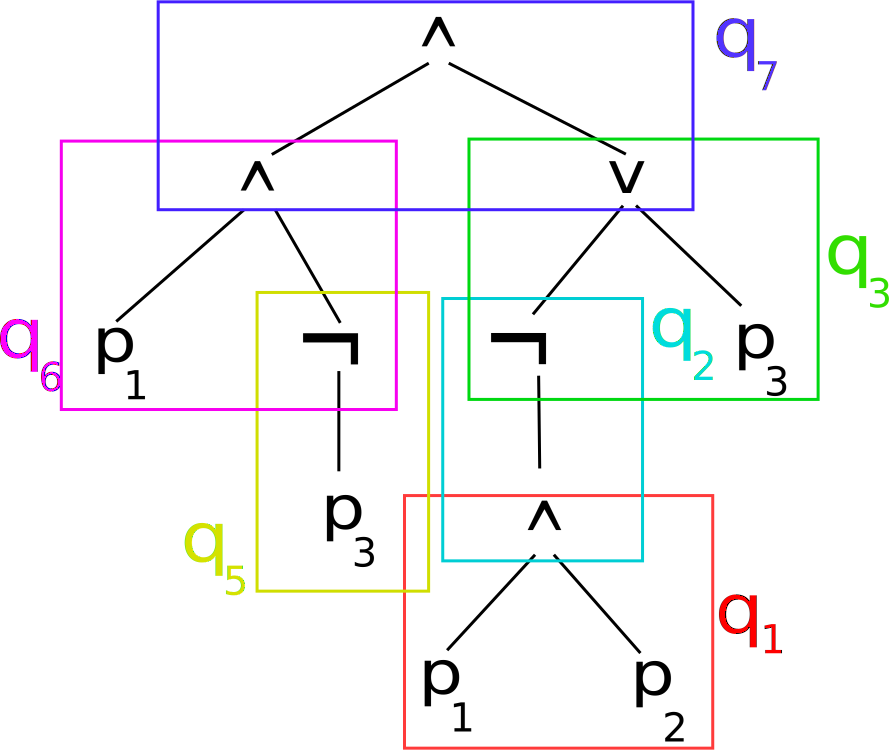
\includegraphics[width=250pt]{arbre_3_FND}
	\end{figure}
	
	$\mathcal{P}=\{p_1, p_2, p_3\}, \mathcal{Q}=\mathcal{P} \cup \{q_1, ... q_7\}$
	
	On pose $G \in \mathcal{F}_{\mathcal{Q}}$ avec : $G=$
	$$\begin{array}{l}
	(q_1 \leftrightarrow (p_1 \land p_2)) \\
	\land (q_2 \leftrightarrow q_1)\\
	\land (q_3 \leftrightarrow (q_2 \land p_3))\\
	\land (q_5 \leftrightarrow \neg p_3)\\
	\land (q_6 \leftrightarrow (p_1 \land q_5))\\
	\land (q_7 \leftrightarrow (q_6 \land q_3))\\
	\land q_7
	\end{array}
	$$
	
	On transforme chaque pseudo-clause $(q_i \leftrightarrow (q_j \lor q_k))$ en une conjonction de 3-clauses équivalentes :
	$$(q_i \leftrightarrow (q_j \lor q_k))$$
	$$(q_i \rightarrow (q_j \lor q_k))\land((q_j \lor q_k) \rightarrow q_i)$$
	$$(\neg q_j \lor q_i)\land (\neg q_k \lor q_i)\land(\neg q_i \lor q_j \lor q_k)$$
\end{myproof}

\part{Compléments}

\section{Calcul propositionnel}

\subsection{Théorème de lecture unique}

\begin{mydef}
	Soient $w_0, w_1=a_1...a_n \in \mathcal{M}$, on dit que $w_0$ est un segment initial de $w_1$, noté $w_0 \subseteq w_1$ si $w_0=a_1...a_i$ avec $1 \leqslant i \leqslant n$, et $w_0$ est un segment propre, noté $w_0 \subsetneq w_1$ si $i < n$.
\end{mydef}

\begin{mylemma}
	Soit $F \in \mathcal{F}$ et $G \subsetneq F$, alors $M \notin \mathcal{F}$
	
	Autrement dit, aucune formule n'est le préfixe d'une autre.
\end{mylemma}

\begin{myproposition}
	On note $o[F]$ le nombre de parenthèses ouvrantes d'une formule $F$ et $f[F]$ pour ses parenthèses fermées.
	\begin{enumerate}
			\item $\forall F \in \mathcal{F}, ~ o[F]=f[F]$
			\item $\forall F \in \mathcal{F}, \forall M \in \Sigma^*, ~ M \subsetneq F \Longrightarrow
			\left\{
			\begin{array}{ll}
				o[M] > f[M], \text{ et donc } M \notin \mathcal{F} & (a) \\
				\textbf{x-ou } M = \neg ... \neg \notin \mathcal{F} & (b)\\
				\textbf{x-ou } M = \varepsilon \notin \mathcal{F} & (c)
			\end{array}
			\right.$
	\end{enumerate}
\end{myproposition}

\begin{myproof}
	Soient $F \in \mathcal{F}$ et $M \subsetneq F$, montrons le second point.
	
	\begin{itemize}
		\item Si $F=\neg G = \neg g_1 ... g_n$
		
		\begin{itemize}
			\item cas (c) : $M=\varepsilon$
			\item cas (b) : $M=\neg$
			\item $M=\neg g_1 ... g_i \subsetneq G, ~ i < n$
			
			alors soit $o[M] = o[g_1...g_i] > f[g_1 ... g_i] = f[M]$, ce qui rentre dans le cas (a)
			
			soit $g_1...g_i = \underbrace{\neg ... \neg}_{i \text{ fois}}$, alors $M=\underbrace{\neg ... \neg}_{i + 1 \text{ fois}}$ : on est encore dans le cas (b).
		\end{itemize}
		
		\item Si $F=(G \circ H) = (g_1 ... g_m \circ h_1 ... h_n)$ et $M \subsetneq F$, soit $M=\varepsilon$ (cas (c)), soit $M \neq \varepsilon$ avec
		
		\begin{itemize}
			\item $M=($ alors $o[M]=1 > f[M] = 0$
			\item $M=(g_1...g_i, ~ 1 \leqslant i \leqslant m$, donc $o[M]=o[g_1...g_i] + 1 > f[M] = f[g_1...g_i]$
			\item $M=(G \circ$ donc $o[M]=1+o[G] > f[M]=f[G]$
			\item $M=(G \circ h_1 ... h_i, ~ 1 \leqslant i \leqslant n$, alors $o[M] = 1 + o[G] + o[h_1...h_i]$
			
			$o[M] = 1 + f[G] + o[h_1...h_i] > f[G] + f[h_1...h_i] = f[(G \circ h_1...h_i] = f[M]$
		\end{itemize}
		
		\item Si $F \in \mathcal{P}, ~ M=\varepsilon$, c'est le cas (c).
	\end{itemize}
	
	\cqfd
\end{myproof}

\begin{myproof}
	Soit $F \in \mathcal{F}$
	
	\begin{itemize}
		\item Si $F \in \mathcal{P}$ pour tout $q \in \mathcal{P} \backslash \{F\}$, $q \neq F$.
		
		$\forall G \in \mathcal{F}, ~ F \neq \neg G$ car $|\neg G| \geqslant 2 > 1 = |F|$
		
		$\forall G, H \in \mathcal{F}, ~ \forall \star \in \{\land, \lor, \longrightarrow\}, ~ (G \star H) \neq F$ car $|F| = 1 < 5 \leqslant |(G \star H)|$
		
		\item Si $F=\neg G$ avec $G \in \mathcal{F}$, pour tout $q \in \mathcal{F}$ on a $q \neq F$.
		
		$\forall H \neq G$ on a $\neg H \neq F$
		
		$\neg G \neq (H \star K)$ pour toute formules $H$ et $G$ et tout opérateur $\star$.
		
		\item Si $F=(G_1 \star G_2)$, supposons $F=(H_1 \circ H_2)$ que l'on réécrit
		
		$$a_1...a_k \star b_1...b_l = c_1...c_m \circ d_1...d_n$$
		
		Montrons $G_1 = H_1$, ce qui impliquera $\star = \circ$ et $G_2 = H_2$.
		
		On est face à l'un des deux cas :
		
		$$(*) ~ \underbrace{a_1 a_2 a_3 ...a_k}_{G_1 \in \mathcal{F}} \subseteq \underbrace{c_1 c_2 c_3 ...c_m}_{H_1 \in \mathcal{F}}$$
		
		$$(**) ~ c_1 c_2 c_3 ...c_m\subseteq a_1 a_2 a_3 ...a_n$$
		
		les deux cas sont symétriques, on suppose $(*)$ et par l'absurde que $G_1 \neq H_1$, c'est à dire $G_1 \subsetneq H_1$, ce qui implique d'après le lemme $G_1 \notin \mathcal{F}$.
		
		On a également $\forall F \in \mathcal{F}, ~ \neg G \neq (G_1 \star G_2)$ et $\forall p \in \mathcal{P}, ~ p \neq (G_1 \star G_2)$.
		
		\cqfd
	\end{itemize}
\end{myproof}

\paragraph{Exercice 3}

Soit $C = \bigwedge_{i \in I} l_i$ et $F$ telle que $C$ soit un impliquant de $F$.

\begin{proofpart}{S'il existe $j$ tel que $C_j$ implique $F$, alors $C$ n'est pas premier}
	Supposons qu'il existe $j$ tel que $C_j$ soit un impliquant de $F$.
	
	$C = C_j \land l_j$ alors si une valuation $v$ est telle que $\overline{v}(C) = 1$, c'est que $\overline{v}(C_j)=\overline{v}(l_j)=1$
	
	Cela signifie que $C$ est un impliquant de $C_j$, $C$ n'est donc pas un impliquant premier de $F$.
\end{proofpart}

\begin{proofpart}{Si pour tout $j$ $C_j$ n'implique pas $F$, alors $C$ est premier}
	
\end{proofpart}

\end{document}